% tuples, lists, dictionaries, aliasing, cloning, mutability
% created by Uwe Schadewald
% modified by Mathias Kuntze and Ahmet Uysal
% Add, handout to documentclass arguments for condensed pdf
\documentclass[presentation, 8pt, mathserif, t]{beamer} % , aspectratio=169
\usepackage[english]{babel}
\usepackage{pgf,graphicx}
\usepackage{amsmath, amssymb}
\usepackage[utf8]{inputenc}
\usepackage{lmodern}
\usepackage{palatino}
\usepackage{multimedia}
\usepackage{pgfpages} 
\usepackage{tikz}
\usepackage{datetime}
\pdfoptionpdfminorversion=5

\usepackage{caption}
\usepackage{subcaption}
% if else
\usepackage{ifthen}
% extend table options
\usepackage{tabularx} 
\usepackage{booktabs}
\usepackage{multicol}
\usepackage{multirow}
\usepackage{eso-pic}  % package to set background image
\usepackage[calc]{picture}

% Packages and stuff for ToDo list like itempoints
\usepackage{pifont}
\newcommand{\cmark}{\ding{51}}%
\newcommand{\xmark}{\ding{55}}%
\newcommand{\open}{$\square$}
\newcommand{\done}{\rlap{$\square$}{\raisebox{1pt}{\large\hspace{1.5pt}\cmark}}\hspace{-2.5pt}}
\newcommand{\wontfix}{\rlap{$\square$}{\raisebox{1pt}{\large\hspace{1.5pt}\xmark}}}
\newcommand{\notsure}{\rlap{$\square$}{\raisebox{0.8pt}{\large\hspace{1.5pt}\textbf{?}}}}



% side bar and footer
\setbeamertemplate{headline}{	
	\leavevmode
	\vspace{-4em}	
	\hbox{		
		\begin{beamercolorbox}[wd=0.85\paperwidth,ht=10ex,dp=8ex,center]{}%			
			% navigation with subsections as dots
			\hspace{3.5em}\insertnavigation{0.7\paperwidth}{\hskip0pt plus1fill} % add navigation in footer						
			% navigation with sections, no subsections
			% \insertsectionnavigationhorizontal{0.6\paperwidth}{\hskip0pt plus1fill}{} \\ % add navigation in footer}
			
		\end{beamercolorbox} 				
	}
	\vskip0pt
}


\setbeamertemplate{footline}{	
	\leavevmode
	\vspace{-3em}
	\hbox{
		\begin{beamercolorbox}[wd=.33\paperwidth,ht=2.25ex,dp=1ex,left]{author in head/foot}%
			\hspace{5em}
			\insertshortauthor
		\end{beamercolorbox}
		\begin{beamercolorbox}[wd=.33\paperwidth,ht=2.25ex,dp=1ex,center]{title in head/foot}%
			\insertshorttitle \ - \insertshortsubtitle
		\end{beamercolorbox}	
		\begin{beamercolorbox}[wd=0.30\paperwidth,ht=10ex,dp=8ex,right]{pagenumber in head/foot}			 	
			\insertframenumber % add page numbers
		\end{beamercolorbox}
	}			
	\vskip0pt
}



\setbeamertemplate{frametitle}{
	\ifthenelse{\equal{\insertframesubtitle}{}}{
		\vspace{0.6cm}
		\huge{\insertframetitle}
	}{
		\vspace{0.6cm}
		\small{\insertframetitle}\\
		\vspace{0.3cm}
		\huge{\insertframesubtitle}
    }		
}

	
% enumerate sections
\setbeamertemplate{section in head/foot}{\hfill\insertsectionheadnumber.~\insertsectionhead}
%\setbeamertemplate{section in head/foot shaded}{\color{structure!50}\hfill\insertsectionheadnumber.~\insertsectionhead}
\setbeamertemplate{section in toc}{\inserttocsectionnumber.~\inserttocsection}

%enumerate subsections
\setbeamertemplate{subsection in head/foot}{\hfill\insertsubsectionheadnumber.~\insertsubsectionhead}
\setbeamertemplate{subsection in head/foot shaded}{\color{structure!50}\hfill\insertsubsectionheadnumber.~\insertsubsectionhead}
%\setbeamertemplate{subsection in toc}[subsections numbered]
\setbeamertemplate{subsection in toc}{\vskip0.5em\leftskip=2em\inserttocsubsection\par}

%--------------------------Common------------------------------------------------------
\setbeamercovered{transparent} % make the beamer theme invisible
\usefonttheme{structurebold}
\beamertemplatenavigationsymbolsempty % set navigations helper function to off
\setbeamertemplate{bibliography item}[text]
\setbeamertemplate{note page}[plain]

%\setlist[itemize,1]{label={$\bullet$}} % \item are using bullets
\setbeamertemplate{itemize items}[circle]
	
	

	
% create a new command to show it on two screens
% I'm using dspdfviewer.
\newcommand{\setDualView} {
	\setbeameroption{show notes on second screen=right}
}

%\AtBeginSection[]{\subsection{}}
\newcommand{\addcite}[1]{%
	\AddToShipoutPictureFG*{%
		\AtPageLowerLeft{%
			\put(0.90\paperwidth,5em){											
				\tiny{
					\cite{#1} 
				}			
			}
		}
	}	
}

% insert a frame with references -> use bibtex
\newcommand{\insertReferenceFrame}[3]{%
	\section{#1}
	\begin{frame}[allowframebreaks]
		\frametitle{#1}
		\bibliographystyle{#2}
		\bibliography{#3}
	\end{frame}	
}

\AtBeginSection[]{\subsection{}}
	





\usepackage{../KU-Beamer-Template/style/koc} 
\usepackage{minted}
\usepackage{upquote}
\usepackage{graphicx}
\usepackage{tikz}
\usetikzlibrary{shapes.symbols,positioning, chains}

\title{KOLT Python}
\subtitle{Containers, Aliasing \& Mutability} 
\newdate{date}{18}{03}{2019}
\date{\displaydate{date}}
\author{Ahmet Uysal}

\titlegraphic{
\includegraphics[scale=0.2]{../KU-Beamer-Template/style/images/logo_kolt.eps}}

\setbeamercovered{invisible} % transparent

\begin{document}
    \maketitle

    \frame{\frametitle{Agenda}\tableofcontents}

    \section{Recap}
        \begin{frame}{Lists}
            \begin{itemize}
                \LARGE
                \item Group values together. \texttt{my\_values = [1, \textquotesingle a\textquotesingle, None]}
                \item You can think of each element as a variable, accessed by \textbf{indexing}
                \item You can do everything you do to variables to list elements:
                    \begin{itemize}
                        \Large
                        \item Assign new values: \texttt{my\_values[0] = 3}
                        \item Use shorthand assignment operators: \texttt{my\_values[1] += \textquotesingle bc\textquotesingle}
                        \item Learn their type: \texttt{type(my\_values[2]) \# => <class \textquotesingle NoneType\textquotesingle>}
                        \item Change their type: \texttt{my\_values[2] = True}
                        \item Compare their value: \texttt{if my\_values[0] == my\_values[1]: ...}
                    \end{itemize}
                \item What happens when we call \texttt{my\_values[3] = 3}? \texttt{\# => \textbf{IndexError}}
            \end{itemize}
        \end{frame}

        \begin{frame}{Indexing}
            \LARGE
            Access elements at a particular index
            \begin{columns}
            \begin{column}{0.5\textwidth}
                \vspace{-5mm}
                \begin{figure}[H]
                    \bigskip
                    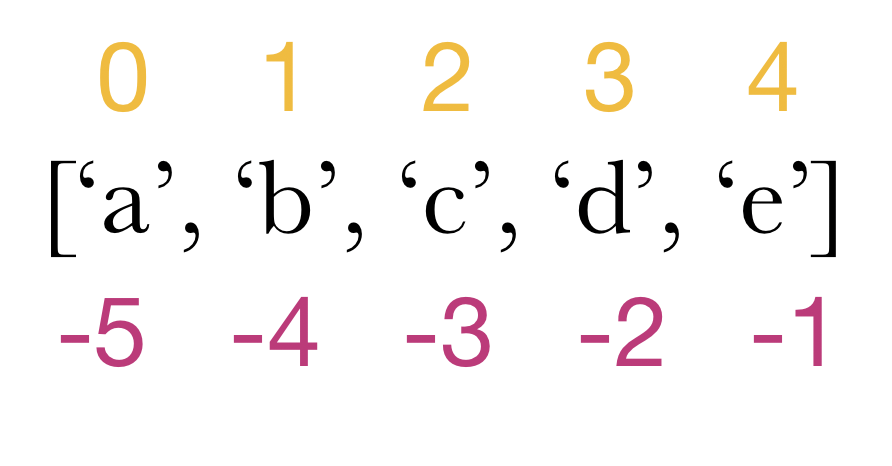
\includegraphics[width=70mm]{../Lecture3/code-examples/index.png}
                    \end{figure}    
            \end{column}
            \begin{column}{0.5\textwidth}
                \inputminted[frame=single,framesep=2pt, lastline=8]{python3}{../Lecture3/code-examples/index.py}
            \end{column} 
            \end{columns}
        \end{frame}

        \begin{frame}{Slicing}
            \LARGE
            Access collection of elements by specifying \textbf{\texttt{[start:stop:step]}}\\
            Gives a list, even when number of elements is not bigger than 1.
            \normalsize
            \vspace{-2mm}
            \begin{columns}
                \begin{column}{0.5\textwidth}
                    \inputminted[frame=single,framesep=2pt,lastline=9]{python3}{../Review1/code-examples/slicing.py}                        
                \end{column}                
                \begin{column}{0.5\textwidth}
                    \inputminted[frame=single,framesep=2pt,firstline=10]{python3}{../Review1/code-examples/slicing.py}                                
                \end{column}
            \end{columns}
            \vspace{2mm}
            \LARGE
            Slices with \texttt{step} = 1 are called \textbf{Basic Slice}.\\
            Slices with \texttt{step != 1} are called \textbf{Extended Slice}.
        \end{frame}

        \begin{frame}{Strings}
            \LARGE
            Special kind of \textbf{lists}! \texttt{name = \textquotesingle Ahmet\textquotesingle\\}
            You can do:
            \begin{itemize}
                \item Indexing: \texttt{name[2]} $\Rightarrow$ \textquotesingle m\textquotesingle
                \item Slicing: \texttt{name[::-1]} $\Rightarrow$ \textquotesingle temhA\textquotesingle
                \item Search by \texttt{in} operator: \texttt{\textquotesingle hm\textquotesingle in name} $\Rightarrow$ \texttt{True}
            \end{itemize}
            You can not do:
            \begin{itemize}
                \item String mutation: \text{name[2]=\textquotesingle H\textquotesingle} $\Rightarrow$ \textbf{\texttt{TypeError}}
            \end{itemize}
            Special functions about strings: \texttt{str.isnumeric(), str.capitalize(), str.format(...), str.find() ...}
        \end{frame}

        \begin{frame}{Loops}
            \LARGE Do something for many elements or based on a condition.
            \begin{columns}
                \begin{column}{0.5\textwidth}
                    \inputminted[frame=single,framesep=2pt]{python3}{../Lecture3/code-examples/while1.py}
                    Similar to simple if blocks, but runs again and again until condition check fails.
                \end{column}
                \begin{column}{0.5\textwidth}
                    \inputminted[frame=single,framesep=2pt]{python3}{../Lecture3/code-examples/for1.py}
                    Iterable: collection of \textbf{ordered} elements.\\
                    What is next after this item?\\
                \end{column}
            \end{columns}
        \end{frame}

        \begin{frame}{For Loops}
            \LARGE
            What is next after this item?\\
            numbers[1] is after numbers[0] \textbf{$\neq$ numbers[1] $>$ numbers[0]}\\
            \textbf{Examples of iterables:} lists, strings, ranges\\
            \huge
            \\
            \textbf{Ranges}\\
            \LARGE
            \texttt{range(start, stop, step)}: creates a sequence of integers from start (inclusive) to stop (exclusive) by step.\\
            Can be \textbf{indexed} and \textbf{sliced}\\
            \texttt{len()} and \texttt{in} operator can be used
        \end{frame}


        \begin{frame}{Break, Continue}
            \begin{columns}
                \begin{column}{0.5\textwidth}
                    \textbf{Break}
                    terminates the closest for or while loop
                    \bigskip  
                    \inputminted[frame=single,framesep=2pt]{python3}{../Lecture3/code-examples/break1.py}
                    \inputminted[frame=single,framesep=2pt]{python3}{../Lecture3/code-examples/break2.py}
                \end{column}
                \begin{column}{0.5\textwidth}
                    \textbf{Continue}
                    continues with the next iteration of the loop
                    \bigskip  
                    \inputminted[frame=single,framesep=2pt]{python3}{../Lecture3/code-examples/continue1.py}
                    \inputminted[frame=single,framesep=2pt]{python3}{../Lecture3/code-examples/continue2.py}
                \end{column} 
            \end{columns}
        \end{frame}
        

    \section{Lists}
    \begin{frame}{List Mutation}
        \LARGE
        \textbf{\texttt{list.append(x)}}: Append x to end of the sequence\\
        \textbf{\texttt{list.insert(i, x)}}: Insert x to index i\\
        \textbf{\texttt{list.pop(i=-1)}}: Remove and return element at index i\\
        \textbf{\texttt{list.remove(x)}}: Remove first occurrence of x\\
        \textbf{\texttt{list.extend(iterable)}}: Add all elements in iterable to end of list\\
        \textbf{\texttt{list[i] = new\_value}}: Update value of index i with new value\\
        \textbf{\texttt{list[basic\_slice] = iterable}}: Change elements in basic slice with elements in iterable, sizes can be different: \texttt{numbers[:] = []}\\
        \textbf{\texttt{list[extended\_slice] = iterable}}: Change elements in extended slice with elements in iterable 1-1, sizes must be equal.\\
    \end{frame}

    \begin{frame}{Some Other List Operations}
        \LARGE
        \textbf{\texttt{in}} operator: Check whether an element is in list. \texttt{3 in numbers} $\Rightarrow$ \texttt{True}\\
        \textbf{\texttt{len(list)}}: Returns the length of list(and other collections).\\
        \textbf{\texttt{list.index(value, start=0, stop=len(list))}}: Return first index of value.\\
        \textbf{\texttt{list.count(value)}}: Count number of occurrences of value in list.\\
        \textbf{\texttt{list.reverse()}}: Reverse the list (in-place)\\
        \textbf{\texttt{list.sort()}}: Sort list elements (in-place)\\
        For more, type \texttt{help(list)} in your interactive interpreter.
    \end{frame}

    \section{Mutability}

    \begin{frame}{Mutability}
        \huge
        \textbf{Immutable:}\\
        \LARGE
        An \texttt{\textbf{object}} with a fixed value.
        \pause
         Immutable objects include \textbf{numbers}, \textbf{strings} and \textbf{tuples}. Such an object cannot be altered.
        \pause
         A new object has to be created if a different value has to be stored.
        \pause
         They play an important role in places where a constant \textbf{hash value} is needed, for example as a \textbf{key} in a \texttt{dictionary}.
        \pause
        \inputminted[frame=single,framesep=2pt]{python3}{code-examples/value_update.py}
    \end{frame}

    \begin{frame}{Python Data Model}
        \pause
        \LARGE
        How did we represent data in Python?
        \pause
         \textbf{Variables!}\\
        \pause
        How do they work?
        \pause
         Do they store the data themselves?
        \pause
        \begin{columns}
            \begin{column}{0.5\textwidth}
                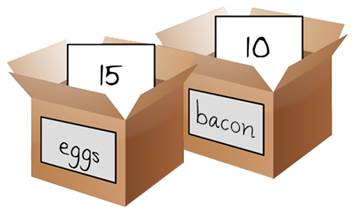
\includegraphics[width=0.9\textwidth]{images/box.jpg}
            \end{column}
            \pause
            \begin{column}{0.5\textwidth}
                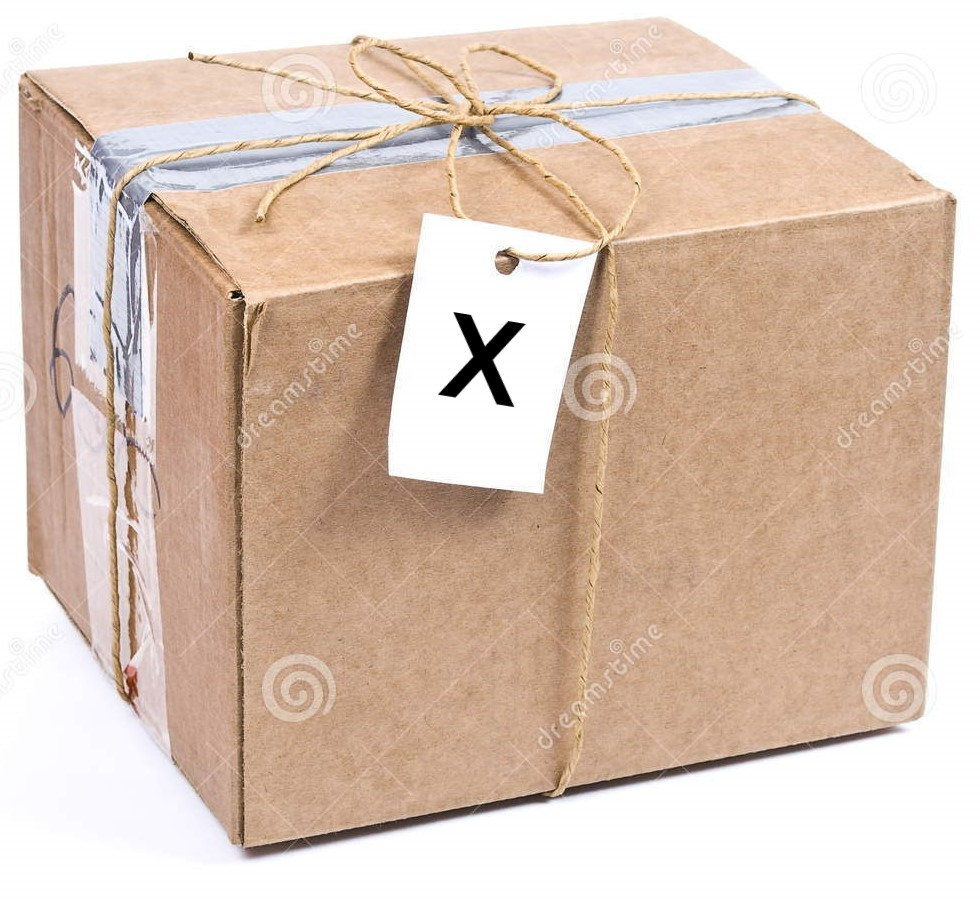
\includegraphics[width=0.6\textwidth]{images/box_tag.jpg}
            \end{column}
        \end{columns}
        
    \end{frame}

    \begin{frame}{Box Analogy}
        \pause
        \LARGE
        \inputminted[frame=single,framesep=2pt,lastline=4]{python3}{code-examples/box_counter_ex.py}
        \pause
        \inputminted[frame=single,framesep=2pt,firstline=6]{python3}{code-examples/box_counter_ex.py}
        \pause
        Did we just changed inside of a closed box?
        \pause 
         Box analogy \textbf{does not} work!
    \end{frame}

    \begin{frame}{Python Data Model}
       \begin{columns}
            \begin{column}[c]{0.5\textwidth}
                \LARGE
                \texttt{my\_secret\_box = [0, 1, 2]}\\
                \visible<5->{\texttt{other\_box = my\_secret\_box}\\}
                \visible<8->{\texttt{other\_box.remove(2)}\\}
                \visible<10->{\texttt{print(my\_secret\_box)}}
            \end{column}
            \begin{column}[c]{0.5\textwidth}
                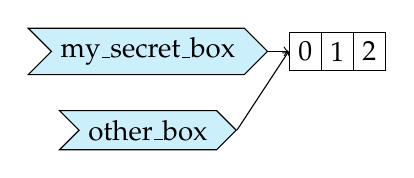
\begin{tikzpicture}%[node distance=-0.15mm]
                    \visible<3->{\node[signal, draw, signal from=west, fill=cyan!20] (var1) {my\_secret\_box};}
                    \visible<2->{
                        \begin{scope}[start chain, right of= var1, node distance=-.5pt, shift={(1,0)}]
                            \def\index{2}
                            \foreach \x in {0,1,2} {
                                \ifx\x\index
                                \visible<2-8>{\node [draw,on chain] (arr\x) {\x};}
                                \else
                                \node [draw,on chain] (arr\x) {\x};
                                \fi
                            } 
                        \end{scope}
                    }
                    \visible<4->{\draw[->] (var1.east) -- (arr0.west);}
                    \visible<6->{\node[signal, draw, signal from=west, fill=cyan!20, below of=var1] (var2) {other\_box};}
                    \visible<7->{\draw[->] (var2.east) -- (arr0.west);}
                \end{tikzpicture}
           \end{column}
       \end{columns}
       \bigskip
       \LARGE
       \visible<11->{Variables are more like \textbf{labels} pointing to \textbf{values}!\\}
       \visible<12->{\textbf{Assignment} links \textbf{variables} to \textbf{values}!}
    \end{frame}


    \begin{frame}{Mutability}
        \huge
        \textbf{Immutable:}\\
        \LARGE
        An \texttt{\textbf{object}} with a fixed value.
        %\pause
         Immutable objects include \textbf{numbers}, \textbf{strings} and \textbf{tuples}. Such an object cannot be altered.
        %\pause
         A new object has to be created if a different value has to be stored.
        %\pause
         They play an important role in places where a constant \textbf{hash value} is needed, for example as a \textbf{key} in a \texttt{dictionary}.
        %\pause
        \inputminted[frame=single,framesep=2pt]{python3}{code-examples/value_update.py}
    \end{frame}

    \begin{frame}{Object}
        \LARGE
        \textbf{Everything} is an object in Python.
        \pause
         Even though variables \textbf{do not} have \texttt{types}, each object has a \textbf{fixed} \texttt{type}.\\
        \pause
        $\hookrightarrow$ Values at the right side of our label analogy are objects!
        \bigskip
        \begin{columns}
            \begin{column}[c]{0.5\textwidth}
                \LARGE
                \visible<4->{\texttt{a = 5}\\}
                \visible<8->{\texttt{a = 10}\\}
                \visible<12->{\texttt{a += 3}\\}
                \visible<16->{\texttt{print(a)}}
            \end{column}
            \begin{column}[c]{0.5\textwidth}
                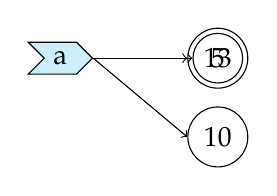
\begin{tikzpicture}%[node distance=-0.15mm]
                    \visible<6->{\node[signal, draw, signal from=west, fill=cyan!20] (var1) {a};}
                    \visible<5-10>{\node[circle, draw, right of=var1, shift={(1,0)}] (val1) {5};}
                    \visible<7-9>{\draw[->] (var1.east) -- (val1.west);}
                    \visible<9-14>{\node[circle, draw, below of=val1] (val2) {10};}
                    \visible<10-13>{\draw[->] (var1.east) -- (val2.west);}
                    \visible<13->{\node[circle, draw, right of=var1, shift={(1,0)}] (val3) {13};}
                    \visible<14->{\draw[->] (var1.east) -- (val3.west);}
                \end{tikzpicture}
           \end{column}
       \end{columns}
    \end{frame}

    \begin{frame}{Object}
        \LARGE
        Each object has an \texttt{identity},
        \pause
         this value can be obtained by using \texttt{\textbf{id()}} function.\\
        \pause
        \textbf{==} operator compares values, \textbf{\texttt{is}} operator compares identities. 
        \pause
        \inputminted[frame=single,framesep=2pt]{python3}{code-examples/identity.py}
        \pause
        Almost always use \textbf{==} to compare values!
    \end{frame}

    \section{Aliasing \& Cloning}
    \begin{frame}{Aliasing \& Cloning}
        \Large
        \begin{columns}
            \begin{column}[c]{0.6\textwidth}
                \begin{itemize}
                    \item More than one variables can refer to \textbf{same object}!
                    \item What if we want to clone/copy instead of aliasing?
                    \item For lists, \texttt{list.copy()} $\Rightarrow$ returns a \underline{shallow copy} of the list.
                    \item Shallow: only copy the references, not inner values.
                    \item \texttt{>>> import copy}
                \end{itemize}
            \end{column}
            \begin{column}[c]{0.4\textwidth}
                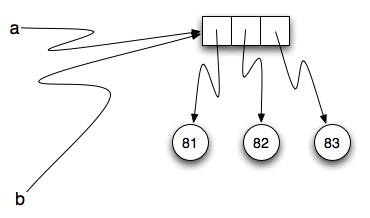
\includegraphics[width=0.9\textwidth]{images/aliasing.png}
            \end{column}
        \end{columns}
        \texttt{copy.copy(x)}: shallow copy, \texttt{copy.deepcopy(x)}: deepcopy   
    \end{frame}


    \section{Tuples}
    \begin{frame}{Tuples}
        \LARGE
        \begin{itemize}
            \item \textbf{Immutable} sequence(ordered) of elements.
            \pause
            \item Similar to \texttt{list}s, you can use \textbf{indexing}, \textbf{slicing}, and iterate over using \texttt{for} loops.
            \pause
            \item Elements cannot be added/removed/changed once the tuple is created.
            \pause
            \item How to create tuples?
            \pause
             \textbf{\texttt{my\_tuple = (1, [1, 2], \textquotesingle a\textquotesingle )}}
            \pause
            \item \textbf{\texttt{len(my\_tuple)}} $\Rightarrow$
            \pause
             3
            \item \textbf{\texttt{my\_tuple.append(3)}} $\Rightarrow$
            \pause
             \textbf{\texttt{AttributeError:}} \texttt{\textquotesingle tuple\textquotesingle \ object has no attribute \textquotesingle append\textquotesingle}
        \end{itemize}
    \end{frame}

    \begin{frame}{Tuples}
        \LARGE
        \texttt{() / tuple()}: empty tuple, 
        \pause
         \texttt{(3)}:
        \pause
         \texttt{int} 3,
        \pause
         \texttt{(3,)}:
        \pause
         \texttt{tuple} containing 3
        \pause
        \inputminted[frame=single,framesep=2pt]{python3}{code-examples/tuples.py}
    \end{frame}

    \section{Sets}
    \begin{frame}{Sets}
        \LARGE
        \begin{itemize}
            \item \textbf{Unordered} \underline{sequence} of \textbf{unique} elements.
            \pause
            \item \underline{\textbf{Cannot}} use \textbf{indexing/slicing}, \textbf{can} iterate with \texttt{for} loops.
            \pause
            \item \textbf{Mutable}, \texttt{add(element)}, \texttt{remove(element)} methods.
            \pause
            \item Python also has \textbf{immutable} sets: \texttt{frozenset}
            \pause
            \item How to create sets? 
            \pause
             \texttt{my\_set = \{1, 2, 3, 4, 2\}}
            \item How to create empty sets?
            \pause
             \texttt{set()} (\{\ \} is reserved for \texttt{dict})
            \pause
            \item Can compute set operations: \textbf{union}, \textbf{intersection}, \textbf{difference}, \textbf{symmetric difference}.
        \end{itemize}
    \end{frame}
    \begin{frame}{Sets}
        \centering
        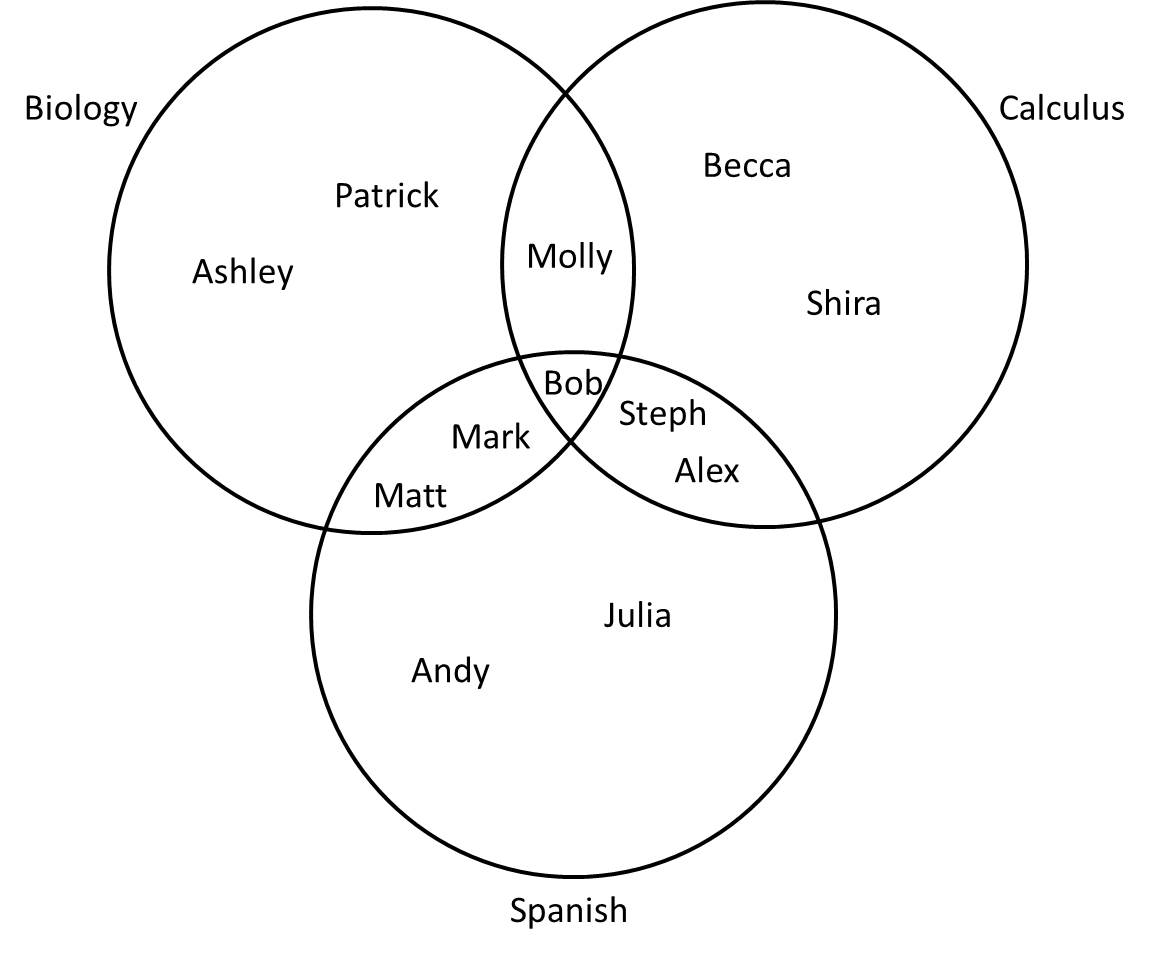
\includegraphics[height=0.75\textheight]{images/venn.jpg}
    \end{frame}
    \begin{frame}{Sets}
        \inputminted[frame=single,framesep=2pt]{python3}{code-examples/sets.py}
    \end{frame}
    \section{Dictionaries}
    \begin{frame}{Dictionaries}
        \LARGE
        \begin{itemize}
            \item Collection of \textbf{key$-$value} \underline{pairs}.
            \pause
            \item \underline{\textbf{Cannot}} use \textbf{indexing/slicing}, \textbf{can} iterate with \texttt{for} loops. 
            \pause
            \item In general, they are not \textbf{ordered}. 
            \pause
            \item However, in Python 3.7 pairs are guaranteed to be in insertion order.
            \pause
            \item In other words, we will get pairs in insertion order if we loop over the \texttt{dict}.
            \pause
            \item How to create dictionaries?
            \pause
             \texttt{\{\ \}/dict()}: empty dictionary
            \pause
            \item \texttt{d = \{\textquotesingle one\textquotesingle : 1, \textquotesingle two\textquotesingle : 2, \textquotesingle three\textquotesingle : 3, \textquotesingle four\textquotesingle : 4\}}
            \pause
            \item How to access values? 
            \pause
             \texttt{print(d[\textquotesingle one\textquotesingle ])} \# $\Rightarrow$ 1
        \end{itemize}
    \end{frame}

    \begin{frame}{Dictionaries}
        \large
        \inputminted[frame=single,framesep=2pt]{python3}{code-examples/dicts.py}
    \end{frame}

\end{document}